\documentclass[a4paper,8pt, twocolumn]{extarticle}
\usepackage[utf8]{inputenc}
\usepackage{graphicx}
\usepackage{tikz}
\usetikzlibrary{arrows,shapes,positioning}
\usepackage[center]{caption}
\usepackage[english]{babel}
\usepackage[top=2.5cm, bottom=2.5cm, left=2.5cm, right=2.5cm]{geometry}

%---------------------------------------------
% Font packages
%---------------------------------------------
% \usepackage{lmodern}
% \usepackage{concmath}
% \usepackage{cmbright}
% \usepackage{kpfonts}
% \usepackage[adobe-utopia]{mathdesign}
\usepackage{fouriernc}
\usepackage[T1]{fontenc}

%---------------------------------------------
% Math environment packages & command
%---------------------------------------------
\usepackage{amsmath}
\usepackage{amssymb}
\usepackage{array}
% \usepackage{mathrsfs}
\usepackage{array}
% \def\sgn{\mathop{\rm sgn}\nolimits} 
% \usepackage{bbm}


%---------------------------------------------
% item option
%---------------------------------------------
\usepackage{enumitem}
%\setitemize{itemsep=0pt}
\renewcommand{\labelitemi}{-}
%\renewcommand{\itemsep}{2em}

%---------------------------------------------
%HEADER & FOOTER
%---------------------------------------------
\usepackage{fancyhdr}
\pagestyle{fancy}

\renewcommand{\headrulewidth}{.15pt}
\fancyhead[C]{{\textsc{The Guarding Problem}}} 
\fancyhead[L]{Page \thepage \ of \pageref{LastPage}}
\fancyhead[R]{DD2438}

\renewcommand{\footrulewidth}{.15pt}
\fancyfoot[C]{\thepage} 
% \fancyfoot[L]{truc}
% \fancyfoot[R]{bidule}

\usepackage{lastpage}

%---------------------------------------------
% two column option
%---------------------------------------------
\setlength{\columnsep}{0.7cm}


%---------------------------------------------
% Table of content
%---------------------------------------------
\usepackage[colorlinks,linkcolor=black, citecolor=black]{hyperref}

%---------------------------------------------
% Opening
%---------------------------------------------
\title{Artificial Intelligence \& Multi-Agent System :\\ \textsc{Artificial intelligence in Real Time Strategy Game}}
%\author{Björn \textsc{Holm}, Kilian \textsc{Demeulemeester} \\ \texttt{\{bjh,kiliande\}@kth.se}}
\author{Björn \textsc{Holm} \\ KTH \\ \texttt{bjh@kth.se}
    \and
Kilian \textsc{Demeulemeester} \\ KTH \\ \texttt{kiliande@kth.se}}
\date{\today}

%---------------------------------------------
% Numerotation Handling
%---------------------------------------------
 %\setcounter{section}{3}
 \usepackage[explicit]{titlesec}
  %\titleformat{<command>}[<shape>]{<format>}{<label>}{<sep>}{<before>}[<after>]
	\titleformat{\section}[block]{\normalsize\bfseries\filcenter}{\Roman{section}.}{1em}{#1}
	\titleformat{\subsection}[block]{\normalsize\bfseries}{\emph{\Alph{subsection}.}}{1em}{\emph{#1}}
 %\titleformat{\section}[hang]{\normalfont\Large\bfseries}%
     %{}{8pt}%
     %{\arabic{section}. #1}


%---------------------------------------------
% Dummy text
%---------------------------------------------
\usepackage{lipsum}

%---------------------------------------------
% Bibliography package
%---------------------------------------------
\usepackage{url}

%---------------------------------------------
% Item package option 
%---------------------------------------------
\newenvironment{shortitem}{
    \begin{itemize}
        \setlength{\itemsep}{0pt}
        \setlength{\parskip}{0pt}
        \setlength{\parsep}{0pt}
    }{\end{itemize}}


%---------------------------------------------
% Algorithm form
%---------------------------------------------
\newtheorem{algorithm}{Algorithm}[section]
\newtheorem{criteria}{Criteria}[section]
\newtheorem{problem}{Problem}
\newtheorem{subproblem}{Problem}[section]
\newtheorem{definition}{Definition}[section]
\newcommand{\qed}{\hfill $\blacksquare$}

\begin{document}

% % Indentation size
% \setlength\parindent{0em}
% 
% \setlength{\itemsep}{0pt}

\maketitle

% \tableofcontents


\begin{bfseries} Abstract -- \end{bfseries}
\emph{
Real Time Strategy games (RTS) present a complete simulated environment that pose many interesting challenges to the research of Artificial Intelligence (AI).
Among these challenges are the huge branching factor of play and constrained time for decision.
In this paper we restrict ourselves the management of military troops at a micro-level, that is: given a scenario with for example 10 vs.\ 10 units that have already discovered each other, which actions should our units perform?
}

\emph{
We describe three different approaches: using scripted behaviors, Alpha-Beta search and UCT search, for unit control in combat scenarios in the game Stacraft: Broodwar, using the Broodwar API (BWAPI) for interfacing with the game \cite{BWAPI}.
}


\vspace{0.5cm}
\hrule

\section{Context}

RTS game provide a very interesting baseground for developping and testing multi-agent cooperative behavior.
Our goal was to create an AI for the \texttt{Stacraft: Broodwar} game. We focused only on the military aspect of the game. Therefore, our bot do not handle harvesting ressources, build order, troops production, \ldots.

We only dealt with the following scenario: Two teams fight against each other with the same number of units (\texttt{Terran Marine}). The goal is to destroy all ennemies units.
This restriction was made in order to test and compare different micro-management algorithm. 
At the current time, we have the following bots:
\begin{shortitem}
\item \texttt{AC: Attack Closest} All units attack their closest opponent,
\item \texttt{ACL: Attack Closest Lethal} All units attack the closest opponent that will not die soon (\emph{i.e} If the amount of damage attributed to this unit is not already enough to kill him soon),
\item \texttt{KS: Kitting Strategy} All units attack their closest opponent applying a kitting\footnote{Staying at a distance, using ranged attacks, and running whenever the enemy comes near} strategy,
\item \texttt{KSL: Kitting Strategy Lethal} All units attack the closest opponent that will not die soon applying a kitting strategy,
\item \texttt{GB: Graph Bot} Heuristic search in the game graph to compute the cleverest action.
\end{shortitem}

\begin{definition}[Scripted based behaviors]
Make decision only on a reactive way and do not make any plan for the future of the game. (Bots \texttt{AC, ACL, KS, KSL})
\end{definition}

\begin{definition}[Heuristic based behaviors]
% TODO
blabla \ldots
\end{definition}


\section{Architecture}

In order to have a huge flexibility in our bot behaviors we designed our AI in a modular and hierarchical fashion (Figure \ref{classDiag}).


\begin{figure}[h!b]
\centering
\begin{tabular}{|c|}
\hline
Commander \\
\emph{Make the overall decision} \\
\hline
\end{tabular} \ \\
\begin{tabular}{c}
$\downarrow$
\end{tabular} \ \\
\begin{tabular}{|c|}
\hline
Squad Manager \\
\emph{Handle $n$ units and lead them into battle} \\
\hline
\end{tabular} \ \\
\begin{tabular}{c}
$\downarrow$
\end{tabular} \ \\
\begin{tabular}{|c|}
\hline
Units \\
\emph{Fight for glory} \\
\hline
\end{tabular}
\caption{Class Diagram}
\label{classDiag}
\end{figure}

Our bot also uses behaviors tree (using the library in \cite{libbehavior}). A example of the behavior tree used by the units acheiving \texttt{Kitting\footnote{Staying at a distance, using ranged attacks, and running whenever the enemy comes near}} is depicted in Figure \ref{behaAttackClos}.

\begin{figure}[h!b]
\caption{Behavior tree for kitting}
\label{behaAttackClos}
\end{figure}

Two differents behaviors has been study for our bot:
\begin{shortitem}
\item Scripted based behaviors
\item Heuristic based behaviors
\end{shortitem}

\begin{definition}[Scripted based behaviors]
Make decision only on a reactive way and do not make any plan for the future of the game.
\end{definition}

\begin{definition}[Heuristic based behaviors]
% TODO
blabla...
\end{definition}

\section{Kiting}
\label{kiting}

Kiting behavior is worth more explanation. 
We based our algorithm on the work of \cite{kiting}. 

\begin{definition}[Kiting]
    Kiting (to kite) is to move units around to make the enemy chase them and thus not be able to attack as much, or not at all. 
    Kiting can be summarize as:
    \begin{shortitem}
    \item Move out of range
    \item Turn back and shoot at the enemy
    \item Repeat
    \end{shortitem}
\end{definition}

The behavior tree used by the units achieving \texttt{Kiting} is depicted in Figure \ref{behaAttackClos}.

\begin{figure}[h!t]
\centering
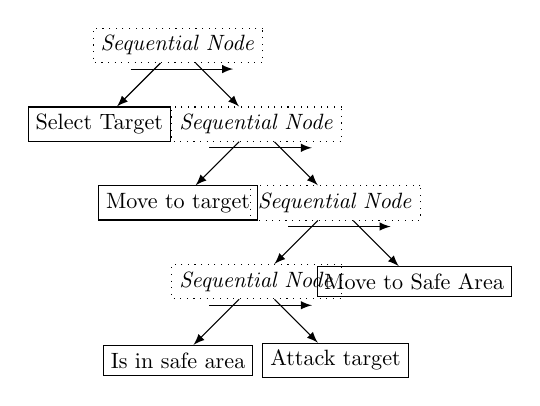
\begin{tikzpicture}[node distance = 1 cm]
    \tikzstyle{leaf}=[rectangle, align=center, scale=0.8, draw]
    \tikzstyle{node}=[rectangle,dotted, align=center, scale=0.8, draw]
    \tikzstyle{tt}=[rectangle,scale=0.8, align=center]
    \tikzstyle{link}=[->,thin,>=latex]
    \node[node] (start) at (1,4) {\emph{Sequential Node}};
    \node[tt] (start1) at (0.3,3.7) {};
    \node[tt] (end1) at (1.8,3.7) {};
    \draw[link] (start1)--(end1);

    \node[leaf] (target) at (0,3) {Select Target};

    \node[node] (seqNode) at (2,3) {\emph{Sequential Node}};
    \node[tt] (start2) at (1.3,2.7) {};
    \node[tt] (end2) at (2.8,2.7) {};
    \draw[link] (start2)--(end2);

    \node[leaf] (leafMove) at (1,2) {Move to target};
    \node[node] (seqAttack) at (3,2) {\emph{Sequential Node}};
    \node[tt] (start3) at (2.3,1.7) {};
    \node[tt] (end3) at (3.8,1.7) {};
    \draw[link] (start3)--(end3);

    \node[node] (attackNode) at (2,1) {\emph{Sequential Node}};
    \node[tt] (start4) at (1.3,0.7) {};
    \node[tt] (end4) at (2.8,0.7) {};
    \draw[link] (start4)--(end4);

    \node[leaf] (moveSafe) at (4,1) {Move to Safe Area};

    \node[leaf] (isSafe) at (1,0) {Is in safe area};
    \node[leaf] (attack) at (3,0) {Attack target};

    \draw[link] (start)--(target);
    \draw[link] (start)--(seqNode);

    \draw[link] (seqNode)--(leafMove);
    \draw[link] (seqNode)--(seqAttack);

    \draw[link] (seqAttack)--(attackNode);
    \draw[link] (seqAttack)--(moveSafe);

    \draw[link] (attackNode)--(attack);
    \draw[link] (attackNode)--(isSafe);
\end{tikzpicture}
\caption{Behavior tree for kiting}
\label{behaAttackClos}
\end{figure}

When selecting the target our bot try to select a target on which a kiting strategy can be used (for instance unit \texttt{A} can not kite another unit \texttt{A}). 
If it can not find any kitable unit then a classic attack is perform (\emph{fight to the death while standing on your position}).

As in paper \cite{kiting} the kiting bot uses an influence map for performing kiting: a 2D matrix $I_{enemy}$.

Let $e$ be an enemy. $e$ has an influence of the area $(i,j)$ of the map if the area can be reached by the enemy before performing kiting.
This relation is denoted $e \textasciitilde (i,j)$.

\begin{multline*}
    e \textasciitilde (i,j) \Leftrightarrow \\ d(e,(i,j)) \leq e.attackRange + e.speed * kitingTime
\end{multline*}

Then the influence matrix is define as:
$$
I_{enemy}(i,j) = \sum_{e \textasciitilde (i,j)}e.DPF \text{ where } DPF = \frac{e.damage}{e.cooldown}  
$$

(DPF is the damage per frame --  average damage of an unit.)

Using this matrix each unit can compute its closest safe position.
Then an attack is performed each time the unit is in a safe area.
Figure \ref{influenceMatrix} shows the influence matrix of a group of 3 units.

\begin{center}
    \begin{figure}[h!t]
        \centering
        \includegraphics[width=0.4\columnwidth]{fig/InfluenceMap.ps}
        \caption{Influence matrix created by a group of 3 units \\ 
        Darker grey means bigger threat}
        \label{influenceMatrix}
    \end{figure}
\end{center}



\vspace{0.5cm}
\hrule
\vspace{0.5cm}
\begin{bfseries} Conclusion -- \end{bfseries}
    \emph{While extremely complicated in term of searchability, RTS game are indeed a solid platform for developing and testing multi agent cooperative behaviors. Our work was focused on micro management and so far we were able to implement some ``classic behaviors'' (\emph{i.e} behaviors used by real human player).} 
    \emph{However, in a future work we want to develop the UCT search and accomplish statistical comparison of the bots. We also aim at improving the bots to fight with 3 kinds of units.} 



\nocite{*}
\bibliographystyle{plain}
\bibliography{bibliography}

\end{document}
